\section{Ejercicio 3}

\subsection{Interpretación del enunciado}
\par{En el piso de un museo se desean instalar sensores l\'aser de seguridad. Cada sensor cubre una determinada cantidad de metros cuadrados del piso. Existen dos tipos de sensores, los sensores bidireccionales de \$4.000 que emiten dos l\'aseres en direcciones opuestas y los sensores cuatridireccionales de \$6.000 que emiten cuatro l\'aseres formando un \'angulo recto entre cada par consecutivo de l\'aseres, es decir, forman una cruz. Cada sensor cubre la posici\'on (x,y) del piso sobre
la que est\'a situado adem\'as de todas las posiciones sobre las que incidan sus l\'aseres. Los l\'aseres bidireccionales pueden ser orientados horizontal o verticalmente. La emisi\'on del l\'aser solo se detiene al alcanzar una pared. Adem\'as de las paredes que delimitan el piso, existen otras paredes dentro del mismo. Los pisos son rectangulares con un ancho y alto determinados. En cada posici\'on (x,y) del piso ($x<ancho$ y $y<alto$) puede haber una pared, un lugar vac\'io o un sensor. No puede haber m\'as de un sensor en la misma posci\'on. Tampoco se puede ubicar un sensor de forma que sea alcanzado por un l\'aser de otro sensor.}
\medskip
\par{Se quiere ubicar alguna cantidad de sensores de forma que toda posici\'on del piso sea vigilada por al menos un sensor. Una posici\'on se considera vigilada si es alcanzada por el l\'aser de alg\'un sensor. Existen adem\'as ciertas posiciones importantes, las cuales deben ser vigiladas por dos sensores distintos. Dado lo costosos que son los sensores, se pide tambi\'en encontrar la forma m\'as barata de vigilar todo el piso. El objetivo de este ejercicio es desarrollar un algoritmo que, dado un piso del museo, determine la forma menos costosa de vigilar cada posici\'on con al menos un sensor (dos las importantes) sin superponer sensores ni que estos se vigilen entre s\'i. Si bien no hay restricci\'on a la complejidad, se pide que el algoritmo desarrollado utilice la t\'ecnica de $backtracking$, y que se implementen podas para reducir el tiempo de ejecuci\'on.}

\subsection{Resolución}
\par{El piso viene representado como una matriz de enteros de dimensiones conocidas. Cada casillero de la matriz se corresponde a una posici\'on del piso y contiene un 0 si hay una pared en dicha posici\'on del piso, un 1 si es un espacio simple (o vac\'io) o un 2 si el espacio es importante. El algoritmo desarrollado realiza backtracking iterativo sobre los casilleros en los cuales se pueden ubicar los sensores, es decir los casilleros en principio vac\'ios. Dado que un casillero importante debe ser vigilado por dos sensores distintos, no tiene sentido ubicar sensores en tales posiciones, ya que tendr\'ia que ubicarse otro sensor en otra posici\'on que vigile esa casilla, pero esto provocar\'ia que un sensor vigile a otro, lo cual est\'a prohibido. Ignorar los casilleros importantes como posibles ubicaciones para los sensores es una primera poda.}
\medskip
\par{Para modelar el problema se tomar\'an los sensores bidireccionales como dos tipos de sensores distintos (aunque con el mismo precio) si se encuentran orientados horizontamente que si se encuentran orientados verticalmente. Entonces se definen tres nuevos posibles valores para cada casillero (uno por cada tipo de sensor). Las posibles soluciones del \'arbol de soluciones del algoritmo consisten en, para cada casillero en principio vac\'io, asignarle un valor correspondiente a alguna de las cuatro posibilidades: que siga vac\'io, que se ubique un sensor horizontal, que se ubique un sensor vertical o que se ubique un sensor cuatridireccional. El total de soluciones es 4^{n}, $con $n$ la cantidad de casilleros en principio vac\'ios. Esta $n$ est\'a acotada por el tama\~no de entrada (el producto entre el ancho y el alto del piso), aunque se considerar\'a la complejidad en funci\'on de dicha $n$. La justificaci\'on para tal decisi\'on es que, como recorrer todas las posibilidades tiene complejidad O(4$^n) $(y backtracking b\'asicamente hace eso) un piso muy grande cubierto de paredes salvo por unos pocos casilleros ser\'a mucho m\'as f\'acil de resolver que uno m\'as peque\~no pero con mayor proporci\'on de casilleros vac\'ios sobre paredes.$}
\par{A continuaci\'on se muestra el pseudoc\'odigo correspondiente al backtracking iterativo sobre los casilleros en principio vac\'ios.}

\begin{algorithm}[H]
	\caption{Resolución basada en Backtracking Ejercicio 3}
	\begin{algorithmic}
		\KwData{Piso $piso$}\\
		Piso $mejor$ \longleftarrow piso\\
		costo($mejor$) \longleftarrow costoMaximo + 1\\
		\While{loop}{
			\If {pisoValido(piso) y costo(piso) < costo(mejor)}{
				$mejor$ \longleftarrow piso
			}
			Casilla $c$ \longleftarrow $primeraCasillaVacia$\\
			$overflow$ \longleftarrow $cambiarValor$(c)\\
			\While{$overflow$} {
				\eIf {$ultimaCasilla$(c)} {
					$loop$ = false\\
					break\\
				} {
					$c$ \longleftarrow $casillaSiguienteVacia$(c)\\
					$overflow$ \longleftarrow $cambiarValor$(c)\\
				}
			}
		}
		\eIf {costo(mejor) > costoMaximo} {
			\textbf{return} No hay solución
		} {
			\textbf{return} $mejor$
		}
	\end{algorithmic}
\end{algorithm}

\par{El piso $mejor$ es el mejor piso encontrado hasta ahora, es decir, la distribuci\'on de sensores m\'as barata. El costo de este piso (la cantidad de dinero necesaria para implementarlo) se inicializa con $costoMaximo$ + 1, para que la primera soluci\'on v\'alida que encuentre, cualqueira sea su costo, lo sobreescriba. Si al finalizar no se encuentra ninguna soluci\'on v\'alida, el costo de la mejor soluci\'on seguir\'a siendo mayor a $costoMaximo$, lo que se utiliza para saber si se debe retornar una soluci\'on, o si no se encontr\'o ninguna (l\'ineas 15 a 18). Al empezar cada iteraci\'on del ciclo principal (l\'inea 3), $piso$ contiene una de las 4^{n} $ soluciones. Lo primero que se hace es verificar si dicha soluci\'on es v\'alida y mejor (m\'as barata) que la \'optima conseguida hasta el momento (l\'ineas 4 y 5). La funci\'on $pisoValido$ recorre todos los casilleros del piso y verifica lo siguiente.$}

\begin{itemize}
	\item Si el casillero est\'a vac\'io, verifica que al menos un sensor vigile su posici\'on.
	\item Si el casillero contiene un sensor, verifica que ning\'un otro sensor vigile su posici\'on.
	\item Si el casillero es importante, verifica que 2 sensores vigiles su posici\'on.
\end{itemize}

\par{La verificaci\'on de cada casillero consiste en recorrer, en el peor caso, toda la fila y toda la columna del casillero, dando una complejidad de O($w$+$h$) con $w$ el ancho y $h$ el alto del piso. Luego la complejidad de la funci\'on $pisoValido$ tiene una complejidad de O($w$*$h$*($w$+$h$)). El resto del ciclo (l\'ineas 6 a 14) cambian el valor de al menos un casillero, obteniendo otra soluci\'on para la siguiente iteraci\'on. La funci\'on $cambiarValor$ toma una casilla y le cambia el valor. El valor puede ser VACIO (no contiene ning\'un sensor), SENSORH (contiene un sensor horizontal), SENSROV (contiene un sensor vertical) o SENSOR4 (contiene un sensor cuatridireccional) y los recorre en ese orden. Cuando se cambia el valor de SENSOR4 a VACIO orta vez, la funci\'on devuelve $true$ para notificar que ya se han probado todas las combinaciones de la casilla, y ahora se debe cambiar el valor de otra casilla. Cuando $cambiarValor$ devuelve $true$ con la \'ultima casilla, significa que ya se han probado todas las combinaciones y el algoritmo debe terminar (l\'ineas 9 a 11). Tanto $primeraCasillaVacia$ como $casillaSiguienteVacia$ recorren la lista de las casillas que en principio est\'an vac\'ias, es decir, incluyendo a las que en ese momento contengan sensores.}
\medskip
\par{Si bien pareciera que el algoritmo funciona a fuerza bruta (probando todas las soluciones posibles), recorre el \'arbol de soluciones al igual que el m\'etodo de backtracking recursivo. Si se considera cada posible soluci\'on como el conjunto de los casilleros vac\'ios donde cada uno puede tomar uno de cuatro valores, entonces cada soluci\'on se puede representar con un n\'umero de $n$ d\'igitos en base 4. Si a su vez se representan en el \'arbol de soluciones de backtracking, se puede establecer una relaci\'on uno a uno entre cada hoja del \'arbol y cada n\'umero en base 4. De esta forma se justifica que el algorimto desarrollado recorre las mismas soluciones que el m\'etodo de backtracking recursivo.}

\subsection*{Podas}
\par{Sin podas, este algoritmo recorre las 4^{n} $ posibilidades. Una primera poda que se implement\'o, adem\'as de la poda trivial de no poner sensores en los lugares importantes, es evaluar, antes de comenzar el ciclo, si alg\'un lugar importante est\'a posicionado de forma tal que no pueda haber 2 sensores vigil\'ando su posici\'on. Como ya se mencion\'o, cada lugar importante debe ser vigilado por un sensor en su misma fila y otro en su misma columna. Entonces, si un lugar importante se encuntra de forma tal que no puede haber ning\'un sensor en su misma fila o en su misma columna, la instancia no tiene soluci\'on posible. La implementaci\'on de esta poda consiste en recorrer cada casillero importante y, de forma similar a la que se verificaba que un casillero sea valido en $pisoValiso$, recorrer su fila y su columna. Si no se encuentra un casillero vac\'io antes de toparse con una pared, en alguna direcci\'on, resulta que la instancia no tiene posible soluci\'on.$}
\medskip
\par{Otra poda implementada consiste en determinar la validez de cada casillero en el momento en que se le asigna determinado valor para reducir la complejidad de $pisoValido$. Por ejemplo, cuando $cambiarValor$ le asigna a una casilla el valor SENSORH (coloca en su posici\'on un sensor horizontal) se asegura que este sensor no est\'e vigilando a otro sensor recorriendo la fila de la casilla. Si es as\'i, intenta asignarle otro valor, en este caso SENSORV, hasta encontrar alguno v\'alido. Esto incrementa la complejidad de $cambiarValor$ ya que debe verificar que el valor que se est\'a asignando es v\'alido. Pero al asegurar que solo instancias v\'alidas (sin sensores apunt\'andose entre s\'i) llegar\'an al principio del ciclo, $pisoValido$, solo debe evaluar que los casilleros sin sensores sean vigilados por alg\'un sensor y que los casilleros importantes sean vigilados por 2 sensores.}
\medskip
\par{Una poda similar consiste en que al entrar en la funci\'on $cambiarValor$, si la casilla es vigilada por otro sensor, no vale la pena probar ubicar sensores en ella. En estos casos se retorna $true$ como notificaci\'on de que ya se han evaluado las cuatro posibilidades, aunque no sea as\'i. Finalmente se implement\'o otra poda para que, si la soluci\'on parcial que se est\'a construyendo es m\'as costosa que la soluci\'on m\'as barata encontrada hasta el momento, se ``retroceda''. Es decir, se dejen vac\'ios todos los casilleros hasta volver a alcanzar un costo temporal menor al de la soluci\'on m\'as barata hasta el momento. Es correcto realizar esta poda debido a que el costo de una soluci\'on parcial (que necesita m\'as sensores para ser una soluci\'on v\'alida) no puede reducirse cuando se alcance una soluci\'on definitiva (cuando termine de agregar los sensores necesarios) ya que agregar sensores s\'olo puede incrementar el costo final.}
\medskip
\par{Las podas implementadas reducen el espacio de soluciones de la misma forma en este algoritmo iterativo como en un backtracking recursivo. Por ejemplo, sea la soluci\'on $A$ = $a_{1}$, $a_{2}$, ... $a_{i-1}$, $a_i$, ... $a_n$, con $a_{j}$ = VACIO $\forall$ j $\in$ (i..n]. Si $a_i$ es VACIO y se va a evaluar asignarle SENSORH (ubicar un sensor horizontal en su casilla), primero se determina mediante la segunda poda enunciada, si tiene sentido hacerlo. Si no es as\'i (si un sensor horizontal en esa posici\'on vigilar\'ia a otro sensor en la misma fila) se deben podar todas las soluciones con el prefijo $A_{1..i}$ = $a_1$, $a_2$, ... $a_{i-1}$, SENSORH. La t\'ecnica de backtracking recursivo realizar\'ia esta poda al recorrer el nodo en el nivel $i$, antecesor de la hoja correspondiente a la soluci\'on A. Dicho nodo es antecesor de todas las hojas cuyas soluciones asociadas tienen el prefijo $A_{1..i}$, entonces al dejar de recorrer esa ramificaci\'on, se evitan evaluar todas esas soluciones. El algoritmo desarrollado con backtracking iterativo realiza la misma poda cuando itera sobre la soluci\'on A. Al comprobar que no tiene sentido asignarle SENSORH a $a_i$, le asigna en su lugar SENSORV, ignorando as\'i todas las soluciones con el prefijo $A_{1..i}$.}

\newpage
\subsection{Complejidad}
\par{A\'un aplicando las podas, la complejidad del algoritmo sigue siendo $O(4^{n})$ ya que en el peor caso, ninguna de las cotas reducir\'ia el conjunto de soluciones y todas ellas deber\'ian evaluarse. Sin embargo, esperamos que en la mayor\'ia de los casos se vea reducido el tiempo total de ejecuci\'on gracias a las podas (es muy com\'un que en un piso haya 2 casilleros vac\'ios adyacentes, caso en el que no se evaluari\'a poner sensores cuatridireccionaoles en ambos). La complejidad de $pisoValido$ sigue siendo O($w$*$h$*($w$+$h$)), ya que debe recorrer todos los casilleros y, para los vac\'ios y los importantes (en la primera iteraci\'on son todos menos las paredes), recorrer una fila y una columna. La funci\'on $cambiarValor$ tambi\'en debe recorrer una fila y una columna pero s\'olo para un casillero (aunque podr\'ia tener que hacerlo 4 veces), por lo que su complejidad es O(4*$w$*$h$). La complejidad final del algoritmo resulta entonces:

\begin{equation}
T(n) = O(4^n*(w*h*(w+h)+4*w*h) = O(4^n*w*h*(w+h+4)) 
\end{equation}

Si acotamos $n$ por $w*h$ y llamamos $s$ a $w*h$, nos queda:

\begin{equation}
T(s) = O(4^s*(ws+hs+4s) = O(4^s*(2s^2+4s)) = O(4^s*s^2)
\end{equation}

Con s la cantidad de casilleros del piso.

\subsection{Implementaci\'on}
\par{Cada piso se representa con una matriz de enteros, donde cada entero representa el contenido de la posici\'on en el piso. Se guardan dos pisos, el $pisoMejor$ (almacena el mejor encontrado hasta el momento) y el $pisoActual$ (el cual se modifica en cada iteraci\'on). La funci\'on $cambiarValor$ toma en un arreglo los casilleros vac\'ios y suma 1 al n\'umero en base 4 que representa a la soluci\'on de $pisoActual$. Ese cambio se ve reflejado en el piso. La funci\'on del pseudoc\'odigo $pisoValido$ se reemplaz\'o en el c\'odigo por $evaluarPiso$ la cual recorre el $pisoActual$ y, si es mejor que el $pisoMejor$, pasa a ser el nuevo $pisoMejor$. Gracias a las podas se sabe que el $pisoActual$ que recorre $evaluarPiso$ es v\'alido en el sentido que no hay sensores apunt\'andose entre s\'i, por lo que s\'olo se asegura que todos los casilleros est\'en siendo vigilados por al menos un sensor y que los casilleros importantes est\'en siendo vigilados por 2 sensores.}
\medskip
\par{La primera poda se ejecuta antes de comenzar el ciclo principal. Para cada casillero importante, se recorren su fila y su columna en busca de alguna posici\'on vac\'ia. Si para alguno no se encuentran, la funci\'on principal retorna sin entrar al ciclo. Las otras podas se implementan en $cambiarValor$ ya que act\'uan al momento de asignar valores a los casilleros. Para determinar la validez de los sensores en los casilleros se implementaron las funciones $vigila(Posicion$ $p)$ que devuelve si un sensor en la posici\'on $p$ est\'a vigilando a otro sensor, $vigilada(Posicion$ $p)$ que devuelve si alg\'un sensor est\'a vigilando la posici\'on $p$ y $doble\_vigilada(Posicion$ $p)$ que devuelve si 2 sensores est\'an vigilando la posici\'on $p$ (utilizada por $evaluarPiso$ para determinar si todas las posiciones importantes est\'an siendo vigiladas por 2 sensores). Estas tres funciones recorren la fila y la columna de la posici\'on $p$ en busca de sensores.}

\newpage
\subsection{Demostraci\'on de Correctitud}
\par{
Para demostrar que es correcto el algoritmo, verificaremos que se cumplen las siguientes propiedades:

\begin{itemize}

	\item El algoritmo sin podas, se fija exhaustivamente (con fuerza bruta) todas las posiblidades, es decir
en las n casillas libres cubriendo todas las posibilidades: que siga vacio, o haya cualquier tipo de sensor. Luego, si hay solución la encuetra y si no, devuelve que no hay solución.
 
	\item Todas las podas son válidas, es decir se saltean casos que no llegan a la solución, o en caso de ser una posible solución 
(que todos los casilleros esten vigilados) seguro no es optima (no es la solución más barata).

\end{itemize}

\Par{Se descarta la posibilidad de instalar sensores en los lugares importantes, ya que si hay un sensor en un casillero importante necesita que lo apunten dos sensores y estos sensores estarían apuntando al sensor instalado, cosa que prohibe el enunciado.
Luego solo es posible agregar sensores en los casilleros vacíos.}

\Par{Podemos pensar a la solución como un número con dígitos $a_0 a_1 ... a_i ... a_n$, en los cuales $(\forall 1 \le i\le n) \quad 0 \le a_i \le 3$.
Donde 0 representa a VACIO , 1 a SENSORH, 2 SENSORV y 3 a SENSOR4.
Cada dígito indica que hay en el casillero i que (en el inicio) estaba vacío.

Veamos que el algoritmo lo que esta haciendo es asignar de izquierda a derecha los números siempre en orden creciente (desde el 0 hasta el 3).
Luego, si no hay ninguna poda, verifica todos los candidatos a solución ($4^n$ candidatos).

Demostración por Inducción (con el algortitmo sin podas):


Hipotesis inductiva: el algoritmo recorre todas las posibles soluciones con n casilleros vacios.
Luego, queremos ver que si tenemos un museo con n+1 casilleros vacios, el algoritmo recorre todas las posibles soluciones.

Caso Base:
El algoritmo cambia el valor de la última y única casilla con las 4 posiblidades (vacío o los tres tipos de sensores). Es decir, tras probar las 4 posibilidades,
 cambiar$\_$valor asigna a la variable $overflow = true $ y entra al ciclo (de $while (overflow)$) y como es la última casilla, asigna loop = false e interrumpe el ciclo. 

Paso inductivo:
\begin{equation}	
	$el algoritmo recorre todas las$  $4^n$ posibles soluciones con n casilleros vacios  $\Rightarrow$ \\
	el algoritmo recorre todas las posibles soluciones con n+1 casilleros vacios. 
\end{equation}

Sea el piso que tiene n+1 casilleros vacíos. Sea una posible solucion el número $A$ = $a_{1}$, $a_{2}$, ... , $a_i$, ... $a_n$ $a_{n+1}$, con $a_i$ un dígito que indica
los 4 posibles estados del casillero. Por la hipótesis inductiva, sabemos que el algoritmo simula los $4^n$ prefijos. Para cada uno de los $4^n$ prefijos el algoritmo 
prueba las 4 alternativas para la última casilla. Por lo tanto prueba las $4^{n+1}$ posibles soluciones.

Esto es porque donde hubiese terminado el ciclo con n casillas, con n+1, $ultimaCasilla$ devuelve false, y se obtiene una casilla más (siendo esta la última de las n+1)
a la que se le cambia una vez el valor y se vuelven a evaluar las $4^n$ posibles soluciones del prefijo que se tenía.
Esto se repite para las 4 opciones que puede tomar la última casilla. 


}

\medskip
\\Ahora demostraremos que las podas son válidas:

\begin{itemize}
\item \par{Alguna más barata : si ya hay una solución con un costo menor al costoMaximo, y se tiene unsa solución parcial con un mayor costo, esta
solución se descarta al igual que toda solución con ese prefijo. 


Demostración: Si $costo(soluciónOptimaDelMomento) \le costoActual(soluciónParcial)$, la solución que tenga como prefijo a la solución parcial, va a tener más o
igual cantidad de sensores, logrando que cualquiera solución con ese prefijo va a ser más cara que la solucionOptimaDelMomento. }

\medskip

\item \par{Si la casilla i está siendo vigilada, ningún número con un sensor(de cualquier tipo) en esa casilla puede ser solución:


Demostración: Cualquier solución que tenga a una casilla i que este siendo vigilada y se le agrega un sensor, este sensor va a tener una señal que impacte al dispositivo agregado, escenario que no puede ser posible por la prohibición del enunciado.
}
\medskip
\item \par{Si una casilla importante se encuntra de forma tal que no puede haber ningún sensor en su misma fila o en su misma
columna, la instancia no tiene solución posible:


Demostración: Sea la casilla i, una casilla importante donde los casilleros que tiene en su misma fila y columnas(hasta llegar a una pared)
son PARED o IMPORTANTE. En este escenario no es posible colocar sensores en las paredes ya que solo se los puede colocar en casilleros libres.
Tampoco se puede colocar en un casillero IMPORTANTE debido a que se apuntarían mutuamente.
}


}

\newpage
\subsection{Testing}
\textbf{Correctitud}\\

Para la realización de los tests de correctitud no haremos muchas variaciones en el tamaño del piso del museo. Consideramos que este aspecto no es muy relevante a la hora de buscar casos bordes.\\

\noindent\textbf{Test$\#$1:} Piso del museo compuesto enteramente por casilleros libres.
\begin{figure}[H]
\centering
\def\svgwidth{140 pt}
\input{imgs/ej3_0.pdf_tex}
\end{figure}
\noindent\textbf{Status:} OK. Se cubren todos los casilleros.\\

\noindent\textbf{Test$\#$2:} Piso del museo compuesto enteramente por paredes.
\begin{figure}[H]
\centering
\def\svgwidth{140 pt}
\input{imgs/ej3_1.pdf_tex}
\end{figure}
\noindent\textbf{Status:} OK. No es necesario ni posible colocar ningun sensor.\\

\noindent\textbf{Test$\#$3:} Todos los casilleros son importantes y necesitan ser cubiertos con 2 sensores.
\begin{figure}[H]
\centering
\def\svgwidth{140 pt}
\input{imgs/ej3_2.pdf_tex}
\end{figure}
\noindent\textbf{Status:} OK. No existe solución\\

\noindent\textbf{Test$\#$4:} Piso cuadriculado.
\begin{figure}[H]
\centering
\def\svgwidth{140 pt}
\input{imgs/ej3_3.pdf_tex}
\end{figure}
\noindent\textbf{Status:} OK. No hay otra posibilidad más que colocar un sensor, vertical u horizontal en cada espacio libre.\\

\newpage
\noindent\textbf{Test$\#$5:} Casilleros importantes en esquinas.
\begin{figure}[H]
\centering
\def\svgwidth{140 pt}
\input{imgs/ej3_4.pdf_tex}
\end{figure}
\noindent\textbf{Status:} OK.\\

\noindent\textbf{Test$\#$6:} Casilleros importantes en el centro.\\
\begin{figure}[H]
\centering
\def\svgwidth{140 pt}
\input{imgs/ej3_5.pdf_tex}
\end{figure}
\noindent\textbf{Status:} OK.\\

\noindent\textbf{Test$\#$7:} Tablero de una sola fila.\\
\begin{figure}[H]
\centering
\def\svgwidth{140 pt}
\input{imgs/ej3_6.pdf_tex}
\end{figure}
\noindent\textbf{Status:} OK.\\

\noindent\textbf{Test$\#$8:} Tablero de una sola columna.\\
\begin{figure}[H]
\centering
\def\svgwidth{140 pt}
\input{imgs/ej3_7.pdf_tex}
\end{figure}
\noindent\textbf{Status:} OK.\\


\newpage
\textbf{Performance}\\
\par{Para este ejercicio, los casos evaluados se realizaron en un conjunto m\'as reducido de instancias, dada la elevada complejidad de la soluci\'on propuesta. Otra particularidad del problema es que la complejidad del algoritmo no crece en funci\'on del tama\~no de entrada (la cantidad de casilleros del piso), aunque s\'i en funci\'on de algo que puede ser acotado por \'el (la cantidad de casilleros en principio vac\'ios). Por ello se decidi\'o generar dos conjuntos de instancias. Primero se generaron instancias en las que cada una se corresponde con una cantidad de casilleros en principio vac\'ios. Luego se generaron instancias en las que cada una se corresponde con el tama\~no del piso. Para el primer conjunto, dada una cantidad $n$ de casilleros vac\'ios se genera un piso de $h$ filas y $w$ columnas con $h = \sqrt{n}$ + 1} y $w = n / \sqrt{n} +1$. Luego se determinaron al azar paredes y posiciones importantes para dejar exactamente $n$ casilleros vac\'ios. Para el segundo conjunto, dado un tama\~no $n$ se genera un piso de $h$ filas y $w$ columnas tal que $h*w = n$. Una vez generados los conjuntos, se ejecutaron ambos y se graficaron los resultados a continuaci\'on.}
\par{El siguiente gr\'afico muestra los tiempos de ejecuci\'on de las instancias generadas para el primer conjunto. Lo que nos importa ver es c\'omo se comporta el algoritmo en funci\'on de la cantidad de casilleros vac\'ios por lo que se grafic\'o en funci\'on de tal. Las series verdes corresponden a las mediciones del algoritmo sin podas, que recorre todas las posibles soluciones, mientras que las series rojas corresponden a la versi\'on del algoritmo que implementa podas. Para cada $n$ cantidad de casilleros vac\'ios, se ejecutaron 50 instancias distintas. Los cuadrados rojos y los c\'irculos verdes son los promedios de las 50 ejecuciones para el algoritmo con y sin podas respectivamente. Cada uno de estos viene acompa\~nado con intervalos verticales que denotan la varianza de cada medici\'on. Tambi\'en se graficaron con cruces rojas y verdes las mediciones m\'aximas y m\'inimas para cada $n$. La curva azul es una funci\'on del tipo $4^n$. Notar que la escala del eje vertical no es lineal sino logar\'itmica.}
\begin{figure}[H]
\centering
\def\svgwidth{140 pt}
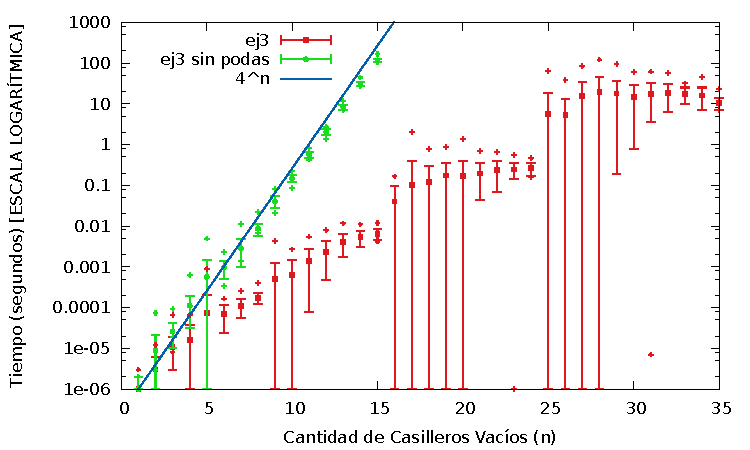
\includegraphics{../codigo/ej3/tests/ej3a.pdf}
\caption{Resultados de las mediciones obtenidas por el script $ej3\_test$ con los par\'ametros 35 1 50 para instancias generadas en funci\'on de la cantidad de casilleros vac\'ios.}
\end{figure}
\par{Lo primero que se puede apreciar en este gr\'afico, es que la complejidad del algoritmo sin podas se ajusta bastante bien a la cota $4^n$ con $n$ la cantidad de casilleros. Si bien esa funci\'on tambi\'en acota los tiempos de ejecuci\'on del algoritmo con podas, estos son considerablemente menores y la diferencia se agranda a medida que aumenta el $n$. La complejidad del algoritmo sin podas parece estabilizarse a medida que se incrementa el tama\~no de entrada (recordar que el tama\~no de entrada fue generado para ser directamente proporcional a la cantidad de casilleros vac\'ios). Esto se deduce al ver como su varianza tiende a achicarse. El algoritmo con podas, por otro lado, parece tener intervalos en los que su complejidad no aumenta demasiado pero luego tiene saltos abruptos. Estos saltos se han identificado en las posiciones correspondientes a valores de $n = k^2$, para $k$ entero (En principio se hab\'ia ejecutado tambi\'en para $n = 36$ pero debido a su excesivo tiempo de procesamiento, se detuvo la ejecuci\'on). Estos valores tienen la particularidad de generar matrices cuadradas (de $\sqrt{n}+1$ x $\sqrt{n}+1$ casilleros). Es tambi\'en en estos saltos en los que se aprecia una mayor varianza, la cual parece disminu\'ir hasta el siguiente salto. Para la mayor\'ia de los valores de $n$, el valor m\'inimo no se ve en el gr\'afico debido a que su tiempo de ejecuci\'on fue tan bajo que se redonde\'o a $0$. Probablemente sean casos en los que, por la primera poda (evaluar si existe una posici\'on importante no vigilable) no se ejecut\'o ninguna iteraci\'on del ciclo principal.}
\par{El siguiente gr\'afico muestra los tiempos de ejecuci\'on de las instancias generadas para el segundo conjunto, es decir en funci\'on del tama\~no de entrada. En este caso, cada una de las $n$ posiciones se determin\'o al azar, aunque favoreciendo la designaci\'on de casilleros vac\'ios para que sean estos los que predominen y no las paredes. Una vez m\'as, las series verdes corresponden a las mediciones del algoritmo sin podas y las rojas al algoritmo con podas. La curva azul es exactamente la misma que la graficada en la figura anterior. Servir\'a para comparar la complejidad del algoritmo en funci\'on del tama\~no de entrada con la complejidad del algoritmo en funci\'on de la cantidad de casilleros. La varianza, los m\'aximos y los m\'inimos fueron graficados de la misma forma que la figura anterior. Tambi\'en con el objetivo de comparar ambas opciones, se mantuvieron las escalas en los ejes.}
\begin{figure}[H]
\centering
\def\svgwidth{140 pt}
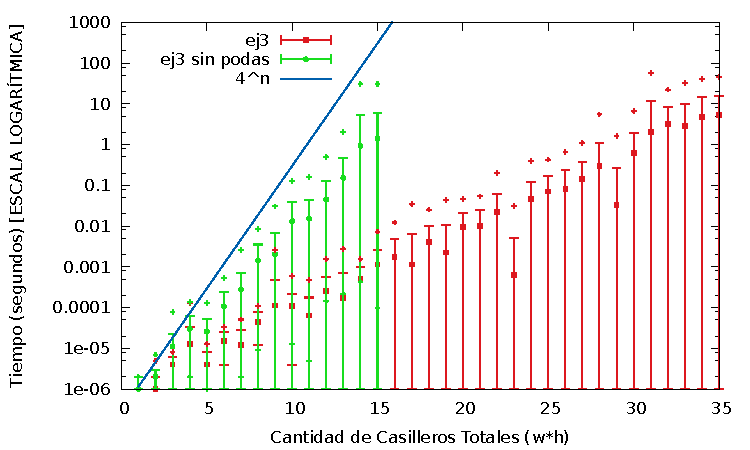
\includegraphics{../codigo/ej3/tests/ej3b.pdf}
\caption{Resultados de las mediciones obtenidas por el script $ej3\_test$ con los par\'ametros 35 1 50 para instancias generadas en funci\'on de la cantidad de casilleros totales.}
\end{figure}
\par{En principio se observa que ambas series est\'an acotadas por la funci\'on que se ajustaba a la complejidad del algoritmo sin podas en funci\'on de la cantidad de casilleros vac\'ios. Incluso el algoritmo sin podas parece crecer con menor complejidad, aunque podr\'ia deberse a que el tama\~no de sus instancias incrementa en 1 para cada valor, mientras que en el caso anterior, incrementar en 1 el valor de $n$ pod\'ia incrementar en m\'as de 1 el tama\'no del piso. Es notable la gran varianza de ambos algoritmos, as\'i como el hecho que que tampoco se graficaron los valores m\'inimos. Todo esto puede ser atribu\'ido a que, dado que no se fijaron la cantidad de casilleros vac\'ios, estos podr\'ian haber sido muy pocos, haciendo muy peque\~no el conjunto de soluciones posibles.}
